\section{Vergleich}
\label{sec:vergleich}

Um einen fairen Vergleich zu ermöglichen, werden alle Implementierungen unter gleichen Bedingungen mit CryptoMiniSat
getestet. Genau wie in Kapitel \ref{chp:bewertung} wird eine Urbildberechnung (siehe Abschnitt \ref{sec:urbildberechnung})
für den Vergleich herangezogen. Die Tests erfolgen jedoch nur von neun bis 21 Bit da die Laufzeit mit einem Thread länger
ist und eine Berechnung für 22 Bit nicht in angemessener Zeit abgeschlossen werden konnte. Außerdem ist pro Bit nur ein
Versuch notwendig, da das Verhalten deterministisch ist und die Laufzeit somit sehr ähnlich. Abbildung \ref{fig:eval_final}
zeigt das Ergebnis des Vergleichs. Zur besseren Übersicht sind die einzelnen Punkte im Diagramm durch Linien verbunden auch
wenn es dazwischen praktisch keine weiteren Messungen gibt.
\begin{figure}[!h]
  \centering
  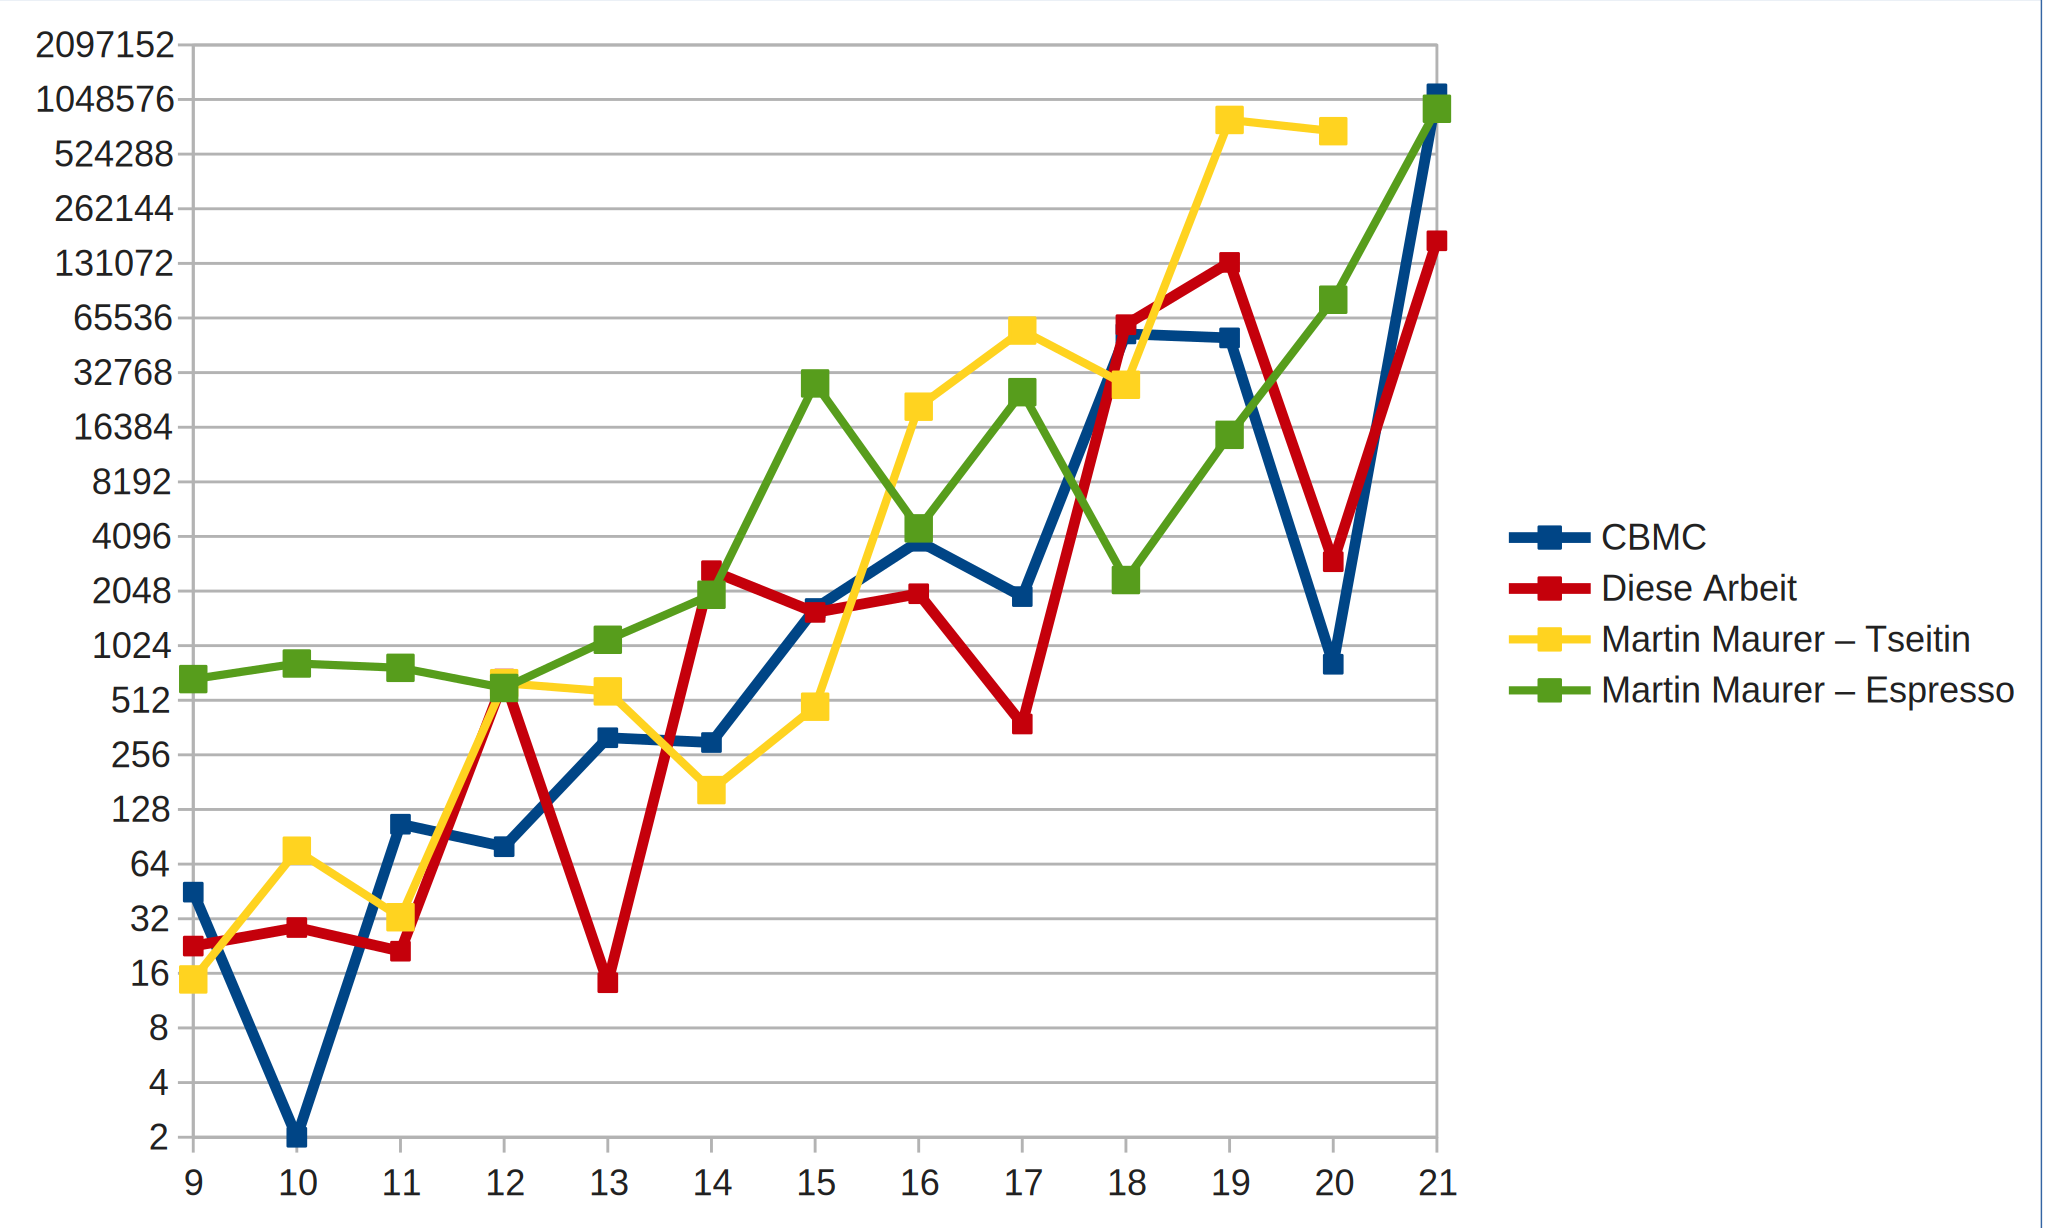
\includegraphics[scale=0.55]{images/eval_final}
  \caption{Eigene Implementierung}
  \label{fig:eval_final}
\end{figure}

Oberflächlich betrachtet hat die in dieser Arbeit erstellte Implementierung mit einer Gesamtdauer von 105 Stunden am besten abgeschnitten.
Die Implementierung von \acr{cbmc} benötigte 344 Stunden. Dieser große Unterschied ergibt sich jedoch ausschließlich aus dem
letzten Test mit 21 Bit. Wird der gesamte Verlauf mit einbezogen, weisen beide Implementierungen ein ähnliches Verhalten auf. Die
Implementierung dieser Arbeit kann an drei Stellen (13, 17 und 20 Bit) vergleichsweise schnell eine Lösung finden während \acr{cbmc} dies
an zwei Stellen (10 und 20 Bit) gelingt.

Die Tseitin-Variante von Martin Maurer verhält sich bis 15 Bit ebenfalls ähnlich, benötigt danach aber wesentlich mehr Rechenzeit.
Inklusive des Versuchs mit 19 Bit benötigt die Tseitin-Variante bereits über 250 Stunden und die Versuche mit 20 und 21 Bit wurden
abgebrochen. Anders verhält sich die Espresso-Variante. Diese benötigt zunächst länger, verhält sich aber ab 16 Bit wieder ähnlich
zur Implementierung dieser Arbeit und \acr{cbmc}. Damit bestätigt sich die Aussage von Martin Maurer, dass in seinen Tests die Tseitin-Variante
schneller war, da er nur Versuche mit einem wenig eingeschränkten Lösungsraum durchgeführt hat. Für die schwierigen Probleme
setzt sich jedoch die Espresso-Variante durch. Für die Tests benötigte diese insgesamt 300 Stunden.